\documentclass[a4paper]{article}
\usepackage[14pt]{extsizes}
\usepackage{setspace,amsmath}
\usepackage{savesym}
\savesymbol{iint}
\usepackage{txfonts}
\restoresymbol{TXF}{iint}
\usepackage[left=20mm, top=20mm, right=20mm, bottom=20mm]{geometry}
\setlength{\parindent}{12,5mm}
\linespread{1.15}
\usepackage[russian]{babel}
\usepackage[T2A]{fontenc} % кодировка
\usepackage{fontspec} 
\defaultfontfeatures{Ligatures={TeX}, Renderer=Basic} 
\setmainfont[Ligatures={TeX,Historic}]{Times New Roman}
\usepackage{graphicx}
\usepackage{lscape}
\graphicspath{{pictures}}
\DeclareGraphicsExtensions{.pdf,.png,.jpg}
\begin{document}
\begin{titlepage}
\begin{center}
\large{Белорусский национальный технический университет}\\
\large{Факультет транспортных коммуникаций}\\
\large{Кафедра «Геодезия и аэрокосмические геотехнологии»}\\
\hfill \break
\hfill \break
\hfill \break
\hfill \break
\hfill \break
\hfill \break
\hfill \break
\large{Отчет\\
 по расчетно $-$ графической работе № 1\\
«Калибровка участка»\\
Вариант №17\\}
\hfill \break
\hfill \break
\hfill \break
\hfill \break
\hfill \break
\end{center}
\begin{flushright}
  \large{Выполнил: ст.гр.11405118\\
	Вишняков М.К.\\
	Проверил: ст. преподаватель\\
	Будо А. Ю.\\}
\end{flushright}
\begin{center}
\hfill \break
\hfill \break
\hfill \break
\large{Минск, 2021\\}
\end{center}
\end{titlepage}
\large{\textbf{Цель работы:} Вычислить параметры преобразования координат из \textit{WGS-84} в плоские местные.
\par Для выполнения поставленной задачи была использована программа «Leica Captivate»
\par \textbf{Исходные данные:} координаты точек в \textit{WGS-84} и местной системы координат. 
\par \textit{Калибровка} $-$ это процесс настройки спроецированных (плоских)
координат в соответствии с местными контрольными координатами. При
калибровке вычисляются параметры для преобразования координат \textit{wgs-proj} в
плоские местные координаты (\textit{NEH}). 
\begin{center}
    \textbf{\textit{Ход работы:}}
\end{center}
\par 1. Открываем программу «Leica Captivate». Далее необходимо создать два проекта.
\par После запуска программы нам открывается главное окно (рисунок 1).
\begin{center}
   \fbox{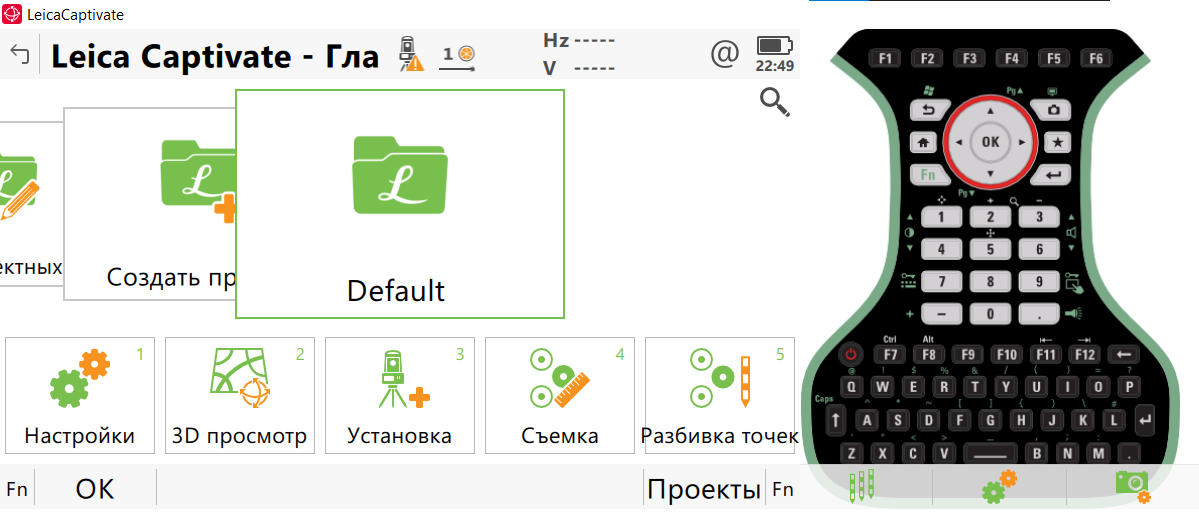
\includegraphics[scale=0.35]{images/1.png} }\\
    Рисунок 1 $-$ Главное окно программы
\end{center}
\par Следующим шагом сама программа предлагает выбрать рабочий проект (рисунок 2), но так как мы работаем в ней впервые необходимо создать новые проекты самостоятельно.
\begin{center}
    \fbox {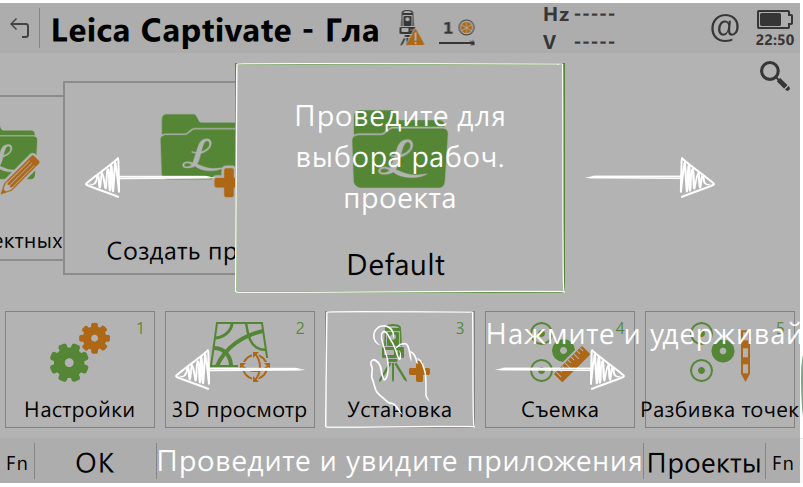
\includegraphics[scale=0.5]{images/2.png}} \\
    Рисунок 2 $-$ Выбор рабочего проекта
\end{center}
\par Нажимаем \textbf{«Создать проект»} $-$ перед нами открывается настройка проекта, в ней мы должны дать имя проекту, а все настройки оставить по умолчанию (рисунок 3) и нажимаем \textbf{«Сохранить»}, аналогичные действия проделываем и со следующим проектом (рисунок 4).
\begin{center}
    \fbox{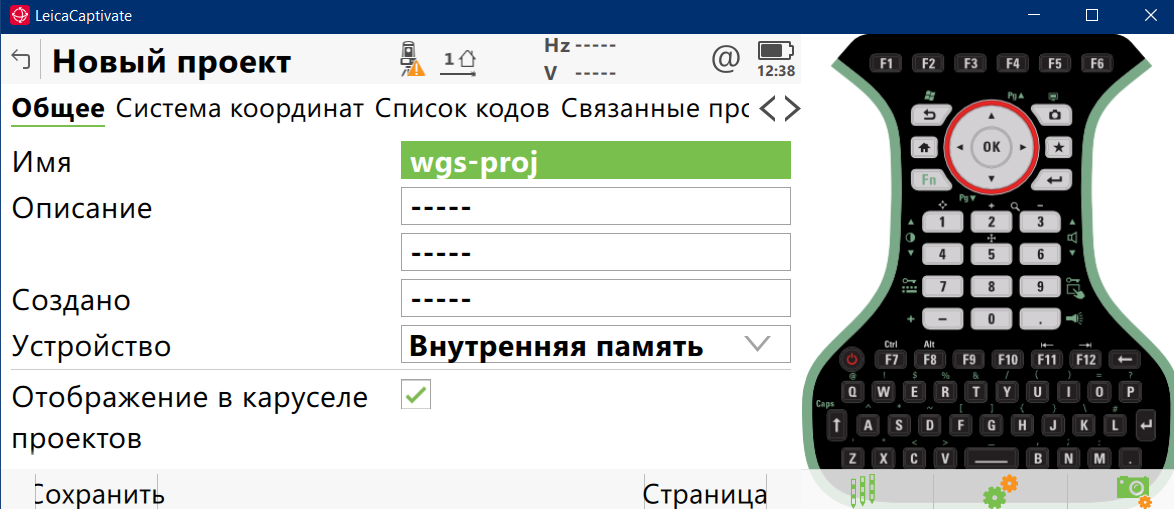
\includegraphics[scale=0.35]{images/3.png}}\\
    Рисунок 3 $-$ Создание проета \textit{wgs-proj} 
\end{center}
\begin{center}
    \fbox{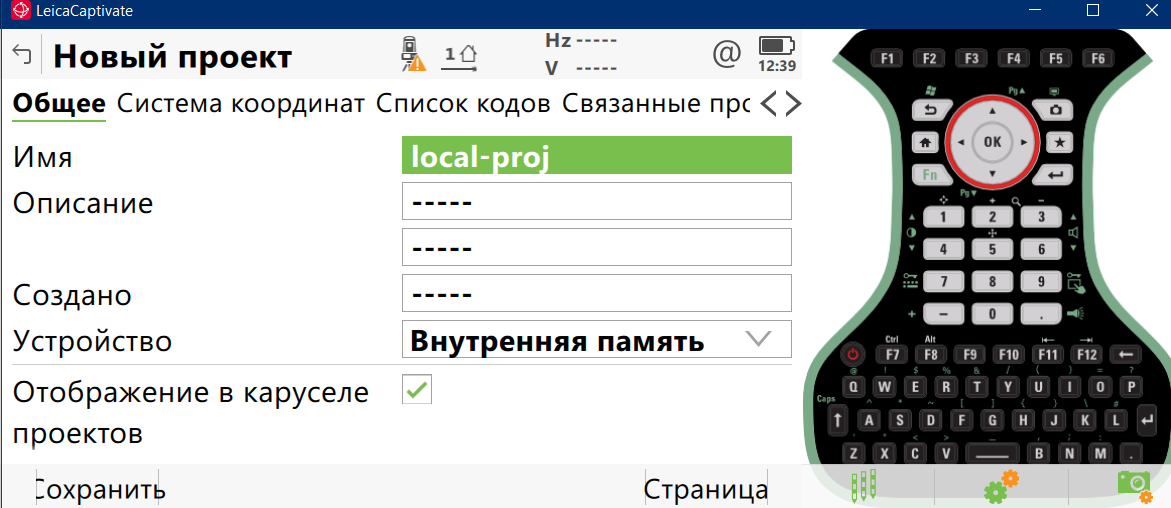
\includegraphics[scale=0.35]{images/4.png}} \\
    Рисунок 4 $-$ Создание проета \textit{local-proj} 
\end{center}
\par 2. Далее предполагается, что мы в одном из этих проектов будем выполнять измерение точек на местности, но так как в симуляторе мы этого выполнить не можем, то координаты пунктов (выданных согластно варианта) будут вводиться вручную. 
\par Для этого: \textbf{«wgs-proj»} → \textbf{«Просмотр и редактирование данных»} → \textbf{«3D просмотр»} → \textbf{«Создать здесь точку»}
\par Последовательность действий представлена на рисунке 5 $-$ рисунке 8.
\begin{center}
   \fbox {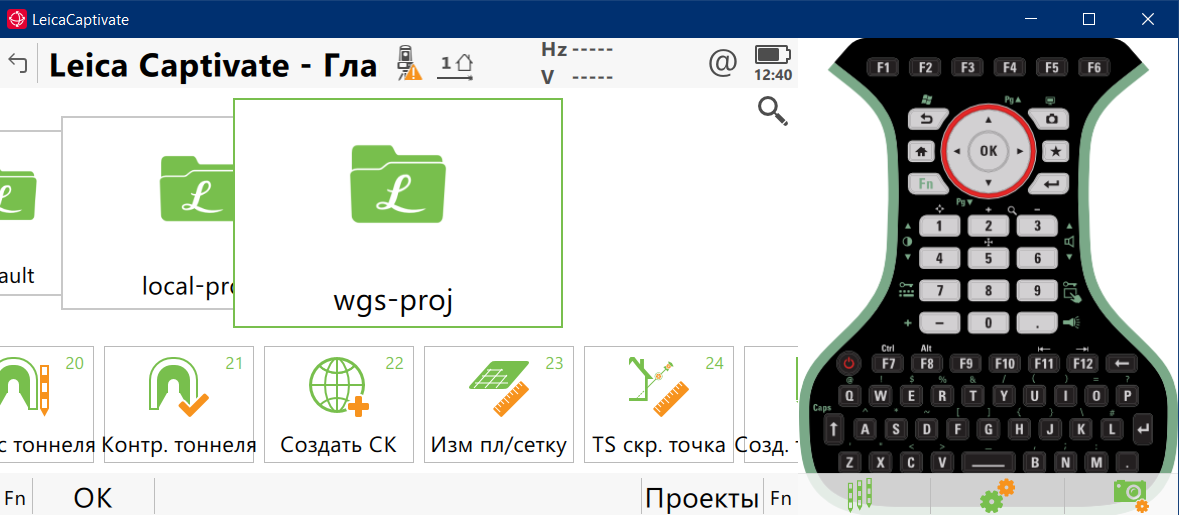
\includegraphics[scale=0.35]{images/5.png}}\\
    Рисунок 5 $-$ Проект \textit{wgs-proj} 
\end{center}
\begin{center}
    \fbox{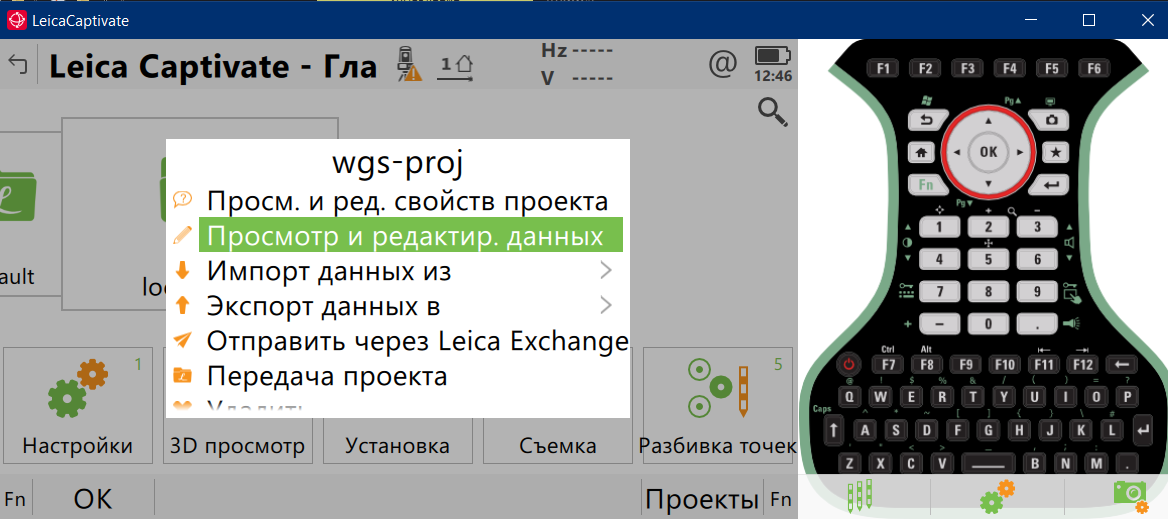
\includegraphics[scale=1.1]{images/6.png}} \\
    Рисунок 6 $-$ «Просмотр и редактирование данных» 
\end{center}
\begin{center}
    \fbox {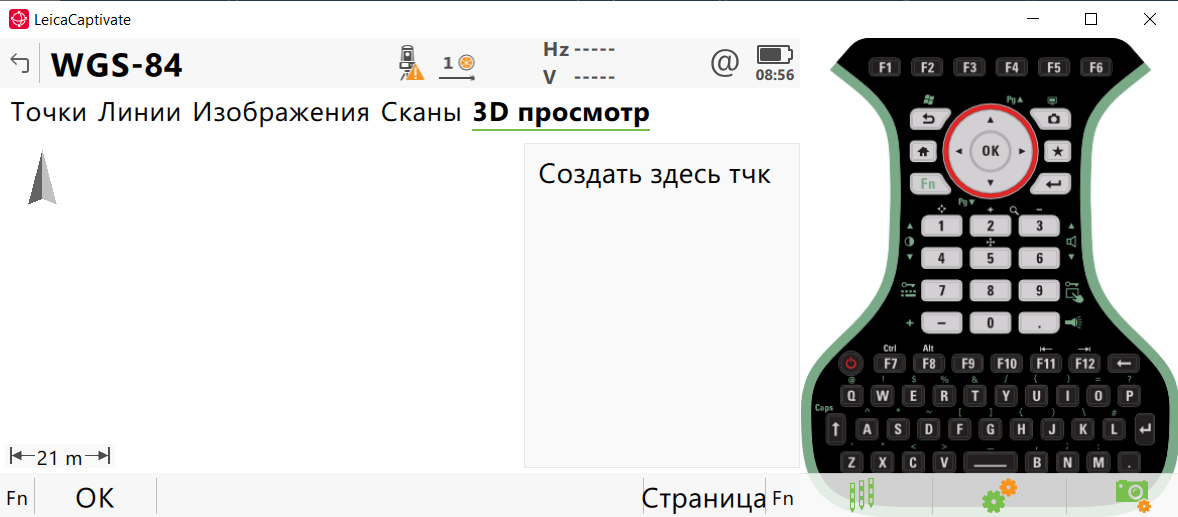
\includegraphics[scale=0.35]{images/7.png} }\\
    Рисунок 7 $-$ «3D просмотр» →\\ «Создать здесь точку»
\end{center}
\begin{center}
    \fbox {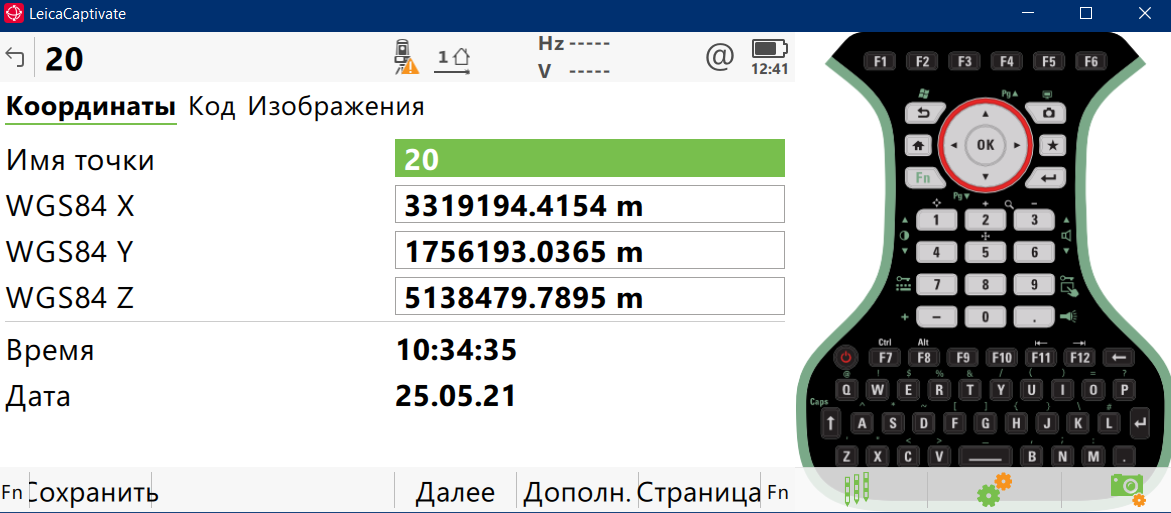
\includegraphics[scale=0.35]{images/8.png}} \\
    Рисунок 8 $-$ Ввод координат точки
\end{center}
\par Но так как в системе по умолчанию заданы плоские прямоугольные координаты, то для ввода долготы и широты необходимо проделать следующие манипуляции: нажимаем \textbf{«Fn»} → \textbf{«Координаты»} → \textbf{«Вводим долготу и широту точки»} → \textbf{«Сохранить»}. \par Последовательность действий представлена на рисунке 9 и рисунке 10.
\begin{center}
    \fbox {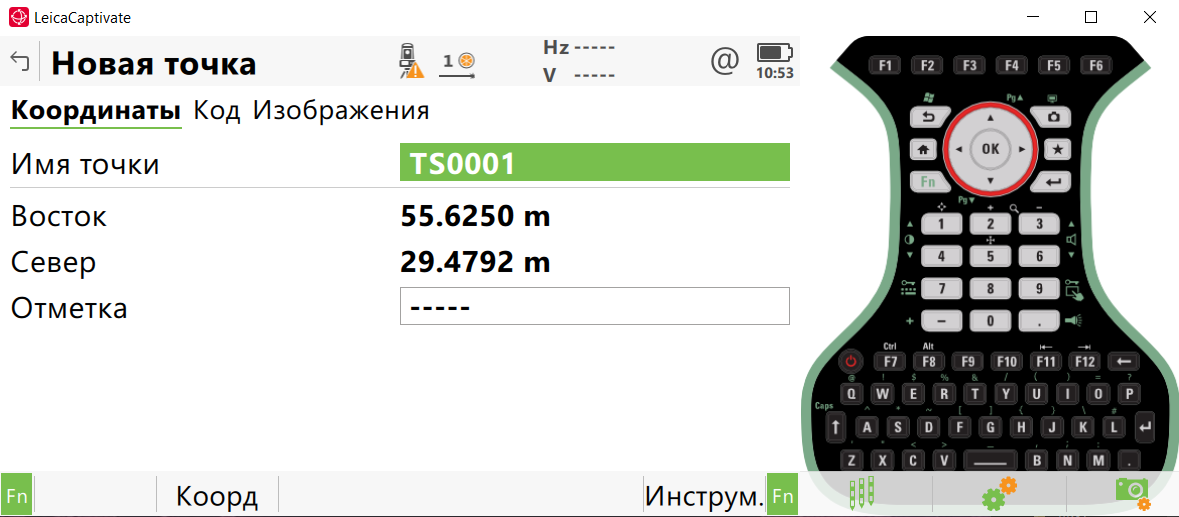
\includegraphics[scale=0.35]{images/9.png} }\\
    Рисунок 9 $-$ «Fn» → «Координаты»
\end{center}
\begin{center}
    \fbox {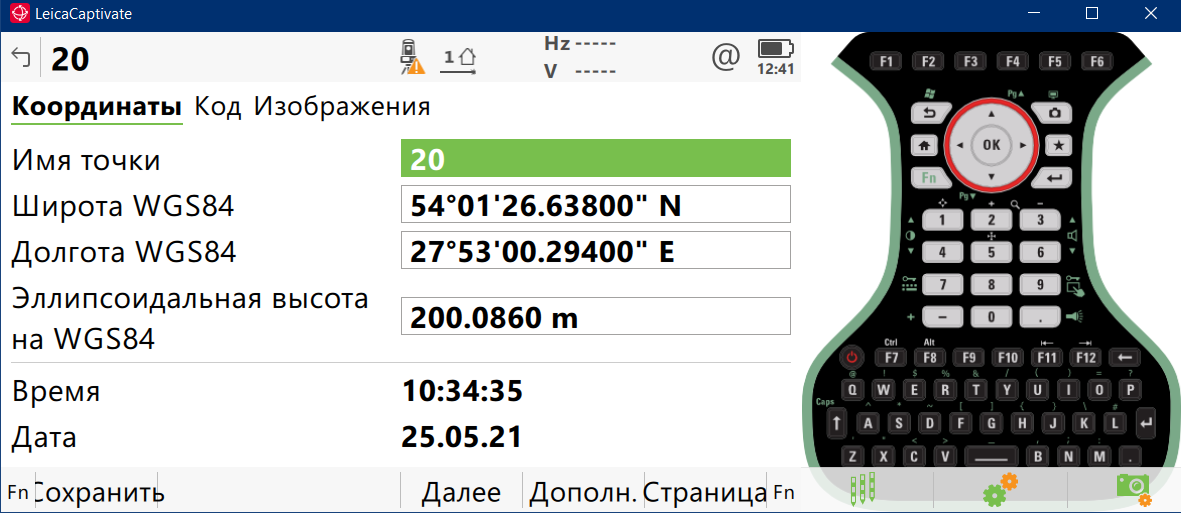
\includegraphics[scale=0.55]{images/10.png} }\\
    Рисунок 10 $-$ «Вводим параметры точки» → \\«Сохранить»
\end{center}
\par Координаты оставшихся точек вводим аналогичным образом.
\par 3. Теперь необходимо ввести данные местной системы координат. 
\par  Ввод данных выполняется в следующей последовательности: \textbf{«local-proj»} → \textbf{«Просмотр и редактирование данных»} → \textbf{«Точки»} → \textbf{«Новый»}→ \textbf{«Сохранить»}
\par Последовательность действий представлена на рисунке 11 $-$ рисунке 14.
\begin{center}
    \fbox {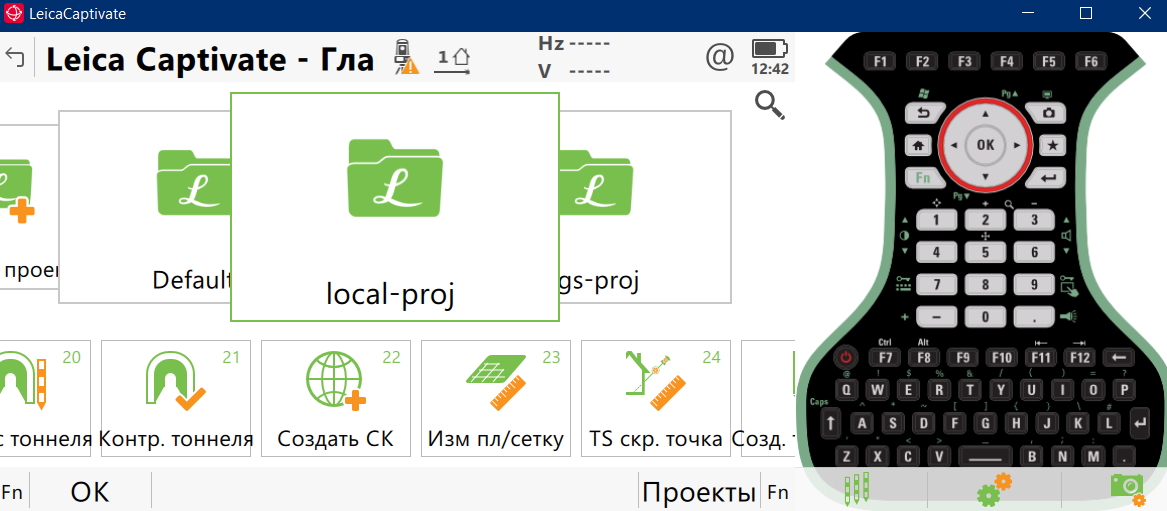
\includegraphics[scale=0.35]{images/11.png} }\\
    Рисунок 11 $-$ Проект \textit{local-proj} 
\end{center}
\begin{center}
    \fbox {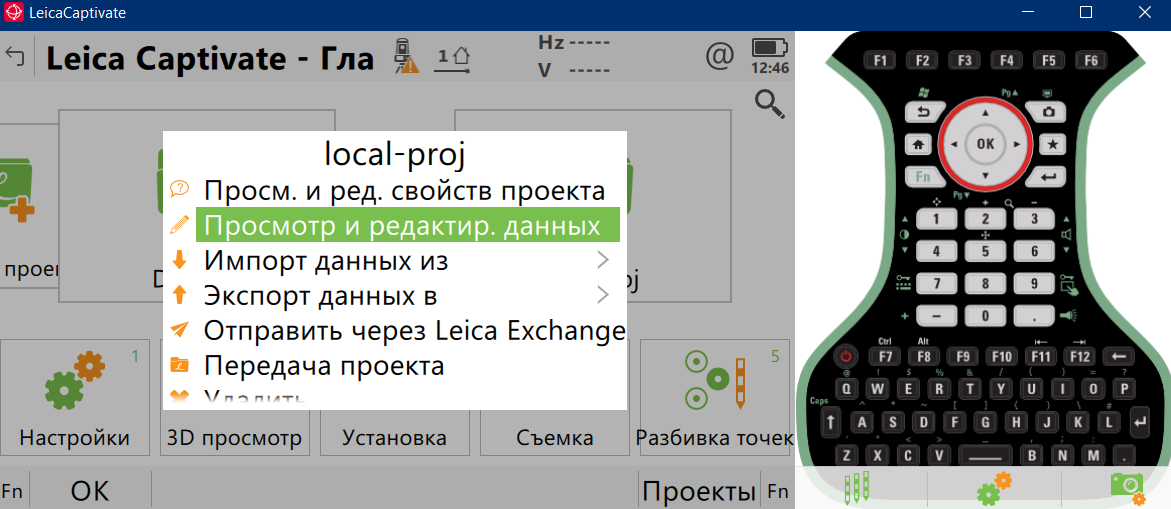
\includegraphics[scale=0.8]{images/12.png}} \\
    Рисунок 12 $-$ «Просмотр и редактирование данных» 
\end{center}
\begin{center}
    \fbox {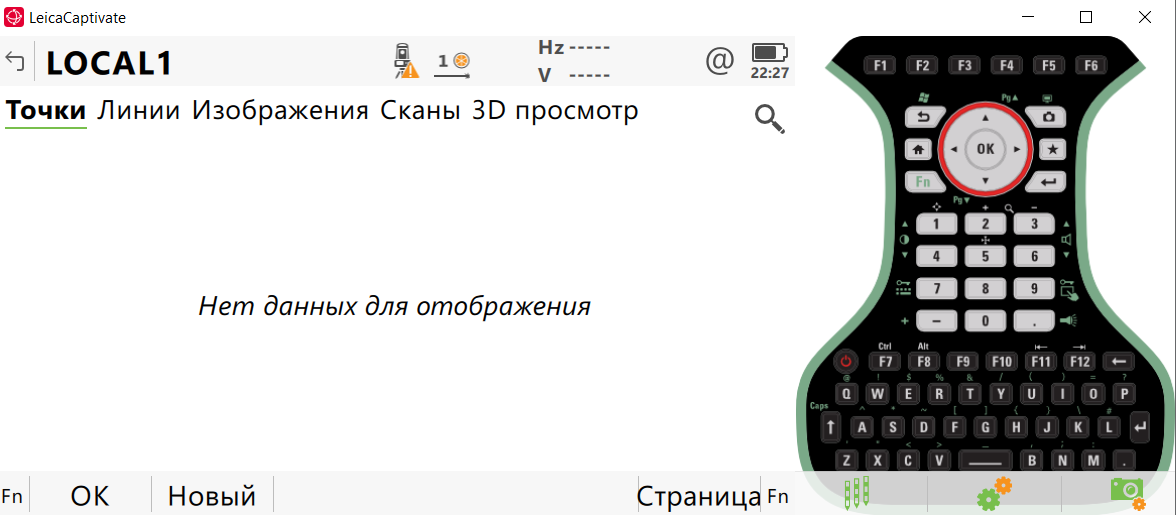
\includegraphics[scale=0.35]{images/14.png} }\\
    Рисунок 13 $-$ «Точки» → «Новый» 
\end{center}
\begin{center}
    \fbox {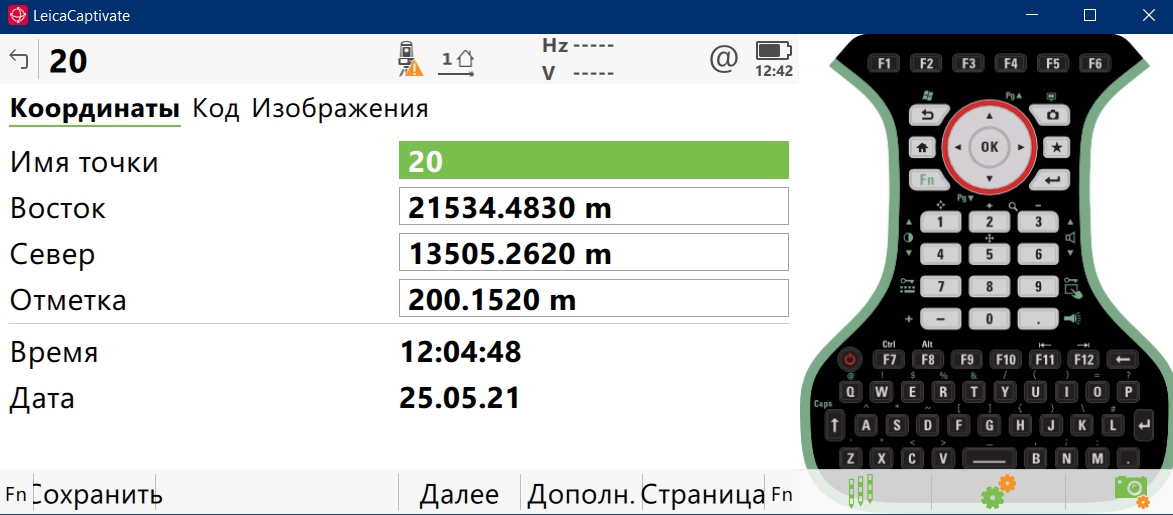
\includegraphics[scale=0.35]{images/13.png} }\\
    Рисунок 14 $-$ «Сохранить»  
\end{center}
\par Координаты оставшихся точек вводим аналогичным образом.
\par Просмотреть расположение точек можно следующим образом: \textbf{«local-proj»} → \textbf{«Просмотр и редактирование данных»} → \textbf{«3D просмотр»} 
\par Последовательность действий представлена на рисунке 15 $-$ рисунке 17.
\begin{center}
    \fbox {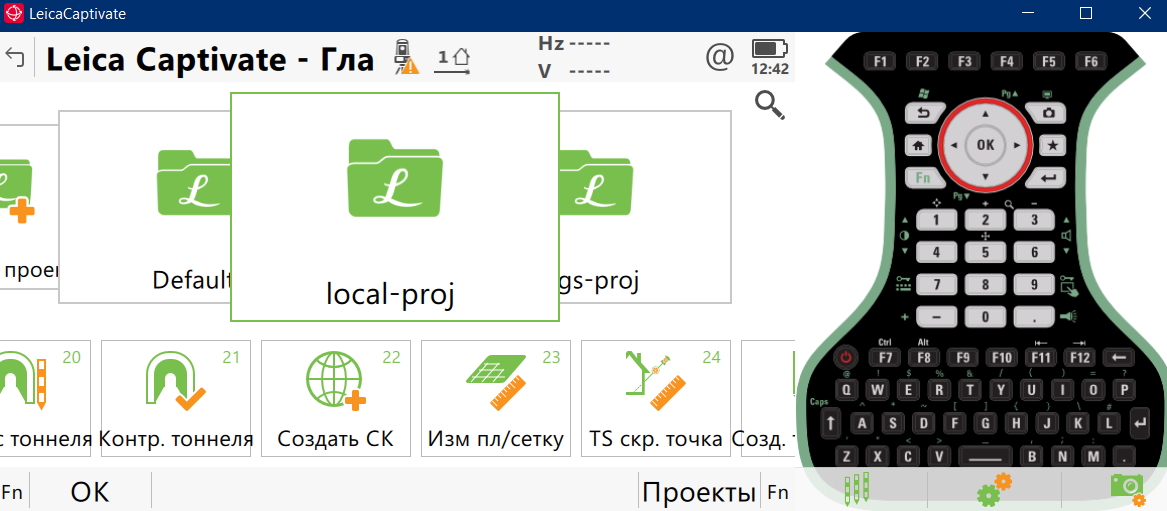
\includegraphics[scale=0.35]{images/11.png}}\\
    Рисунок 15 $-$ Проект \textit{local-proj}  
\end{center}
\begin{center}
    \fbox {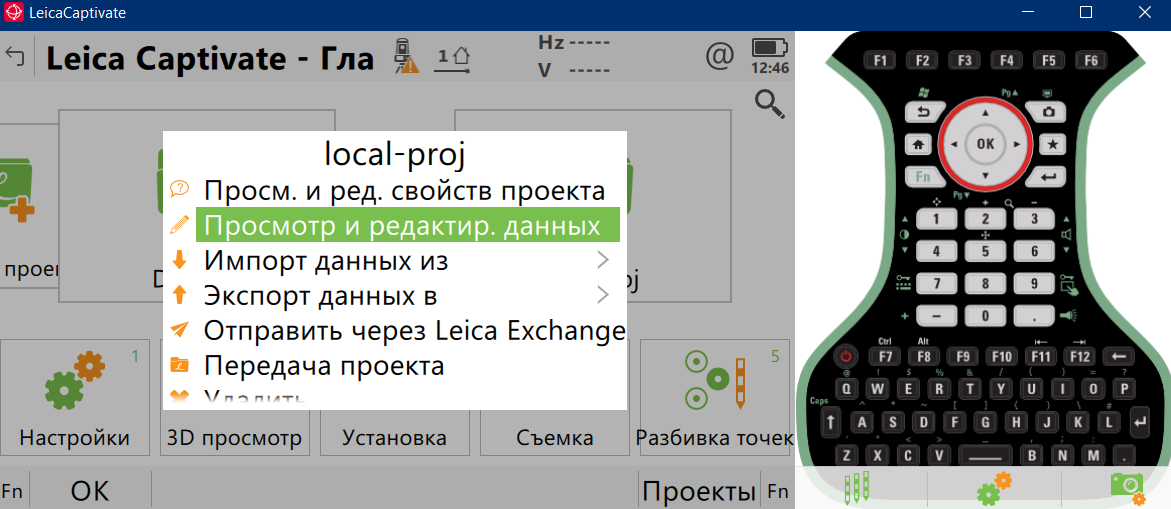
\includegraphics[scale=0.8]{images/12.png}} \\
    Рисунок 16 $-$ «Просмотр и редактирование данных»  
\end{center}
\begin{center}
    \fbox {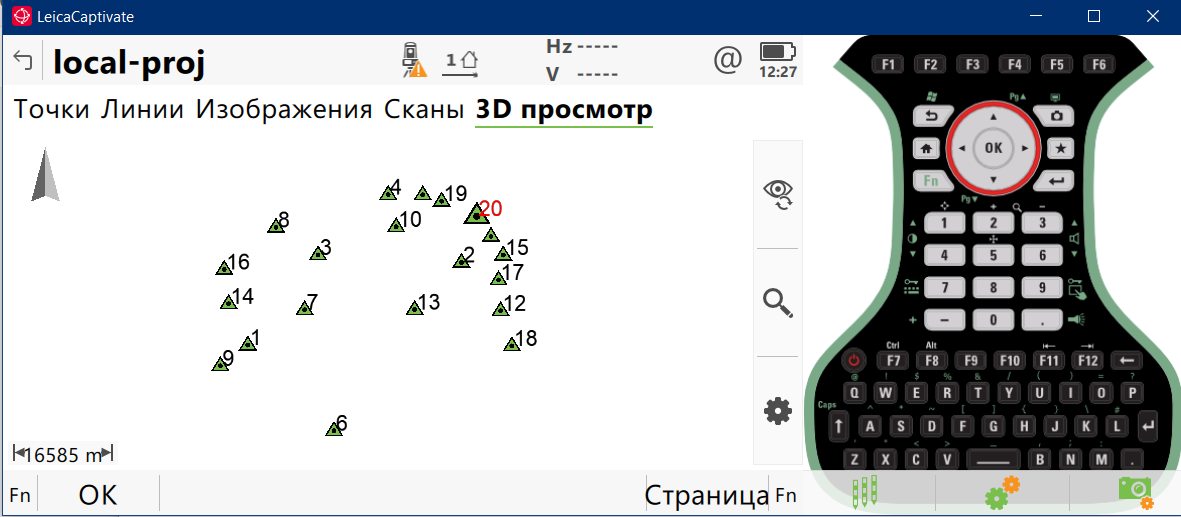
\includegraphics[scale=0.35]{images/15.png} }\\
    Рисунок 17 $-$ «3D просмотр»  
\end{center}
\hfill \break
\par 4. Следующим этапом будет выполнение самой калибровки. 
\par Для нее необходимо в главном меню найти команду систему координат (рисунок 18).
\begin{center}
    \fbox {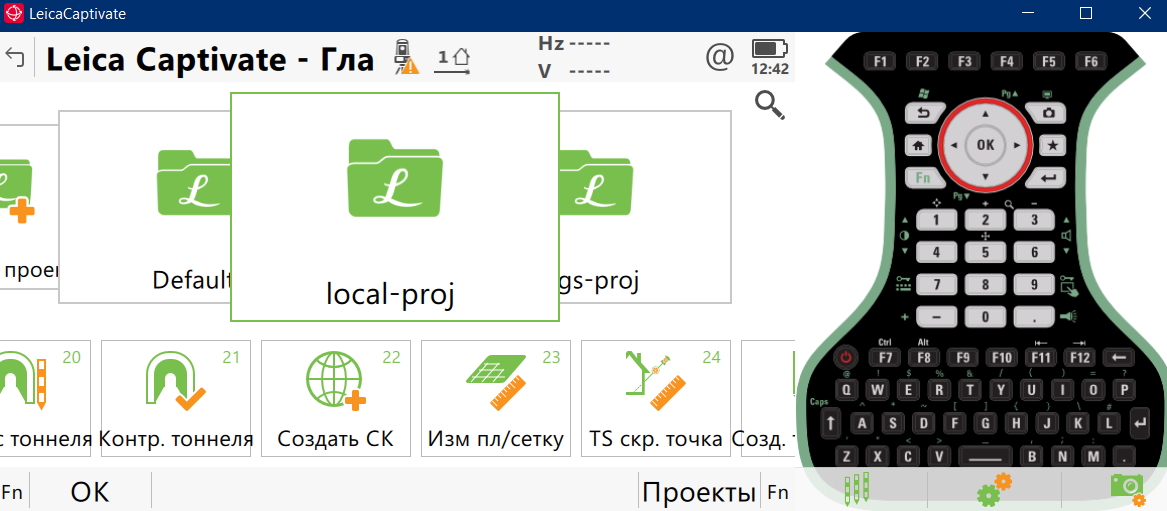
\includegraphics[scale=0.35]{images/18.png}}\\
    Рисунок 18 $-$ «Система координат»  
\end{center}
\par Далее можем выбрать один из методов выполнения калибровки. В нашем случае рациональнее будет использоваться метод \textit{«1 Шаг»} (рисунок 19). 
\begin{center}
    \fbox {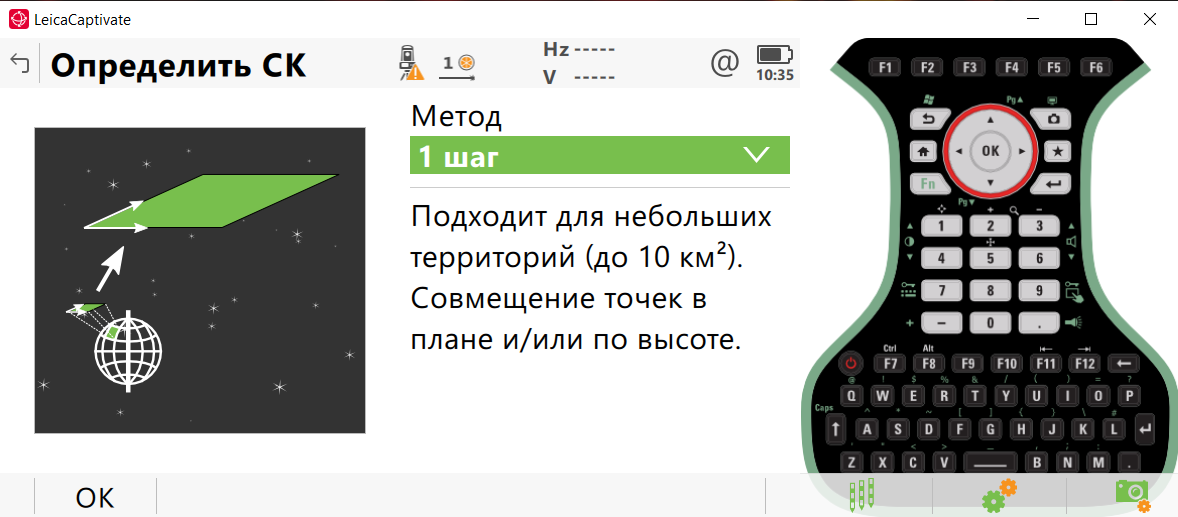
\includegraphics[scale=0.35]{images/19.png} }\\
    Рисунок 19 $-$ \textit{«1 Шаг»}  
\end{center}
\par Создаем проект и указываем проекты с точками \textit{«wgs-proj»} и  (\textit{«local-proj»}) (рисунок 20).
\begin{center}
    \fbox {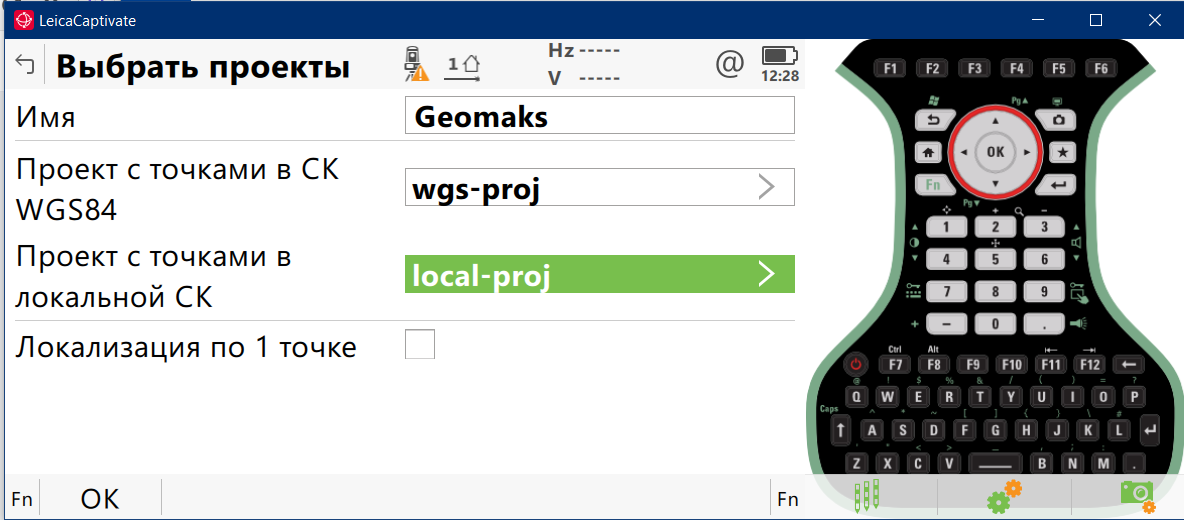
\includegraphics[scale=0.35]{images/20.png} }\\
    Рисунок 20 $-$ Проект для калибровки  
\end{center}
\par Следующим шагом будет выбор типа высот, мы же выбираем эллипсоидальную (рисунок 21).
\begin{center}
    \fbox {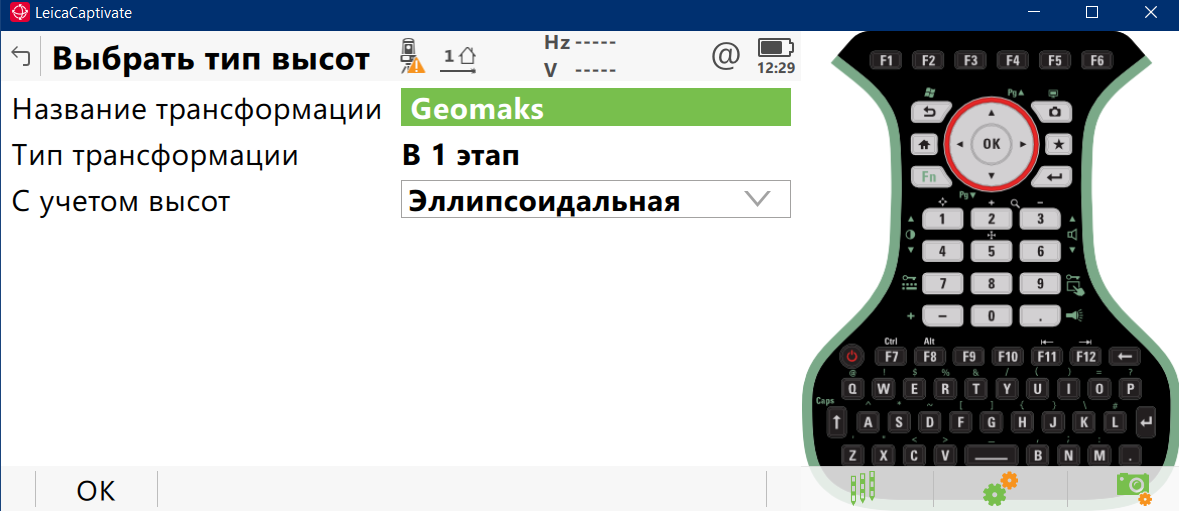
\includegraphics[scale=0.35]{images/21.png}}\\
    Рисунок 21 $-$ Выбор типа высоты  
\end{center}
\par Модель геоида оставляем по умолчанию (рисунок 22).
\begin{center}
    \fbox {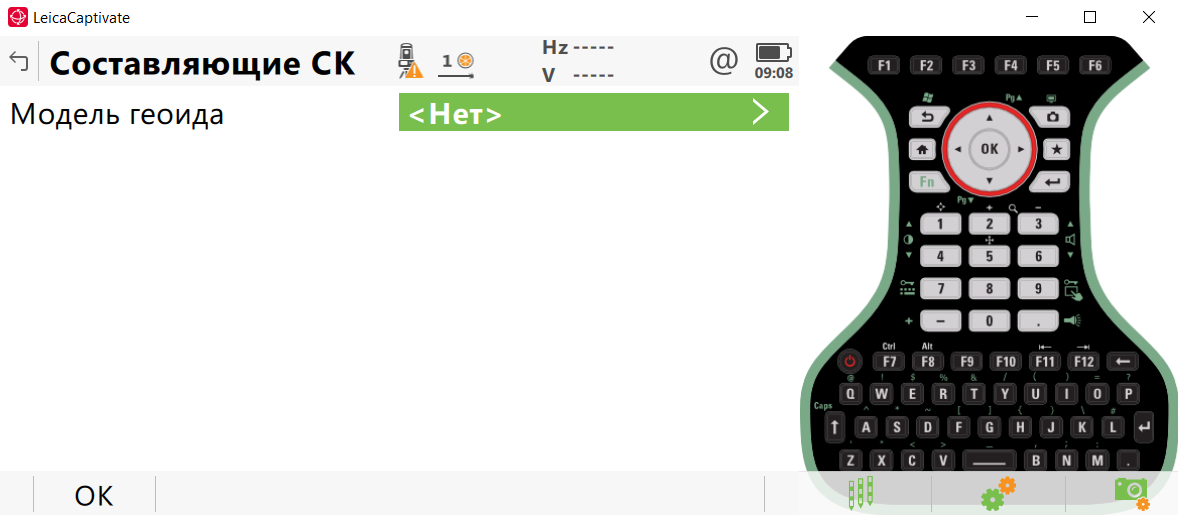
\includegraphics[scale=0.35]{images/22.png}} \\
    Рисунок 22 $-$ Модель геоида  
\end{center}
\par Теперь необходимо связать точки из двух проектов в плане и по высоте (рисунок 23). 
\begin{center}
    \fbox {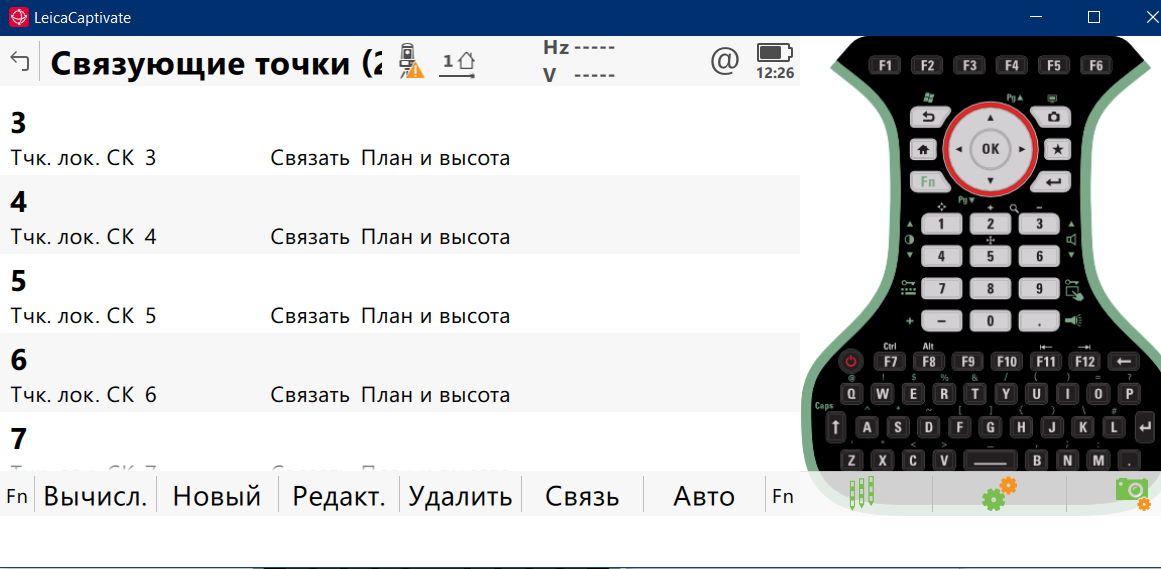
\includegraphics[scale=0.35]{images/23.png}} \\
    Рисунок 23 $-$ Связь точек двух проектов  
\end{center}
\par Выполняем вычисление нажав на «Вычисл.» 
\begin{center}
    \fbox {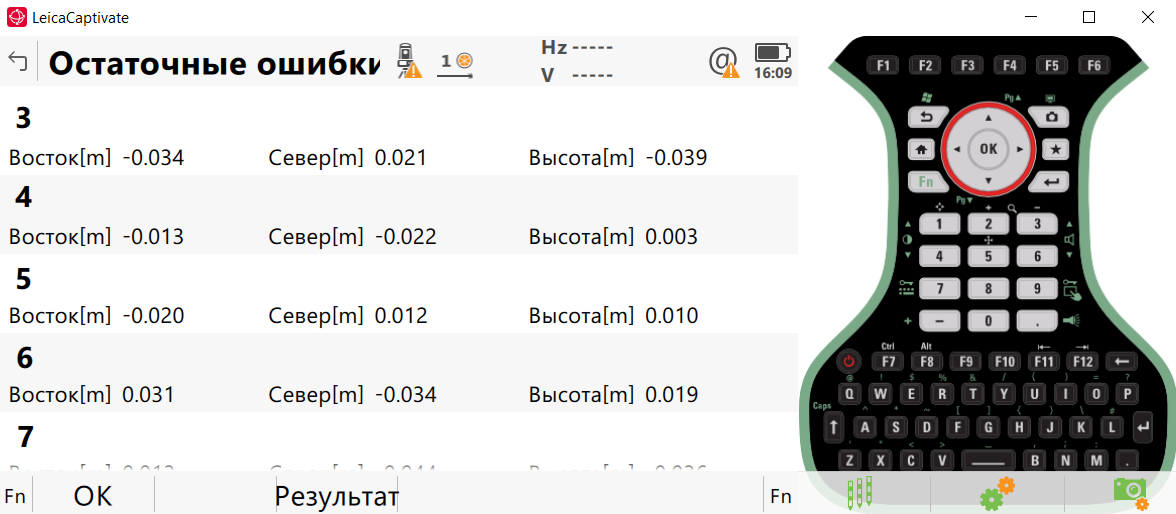
\includegraphics[scale=0.35]{images/24.png}} \\
    Рисунок 24 $-$ Остаточные ошибки  
\end{center}
\par Обращаем внимание на отклонения. Наибольшее отклонения по координате N (север) имеет точка 7, наибольшее отклонения по координате E (восток) имеет точка 9 и наибольшее отклонение по высоте имеет точка 10. 
\par Результат представлен на рисунке 25.
\begin{center}
    \fbox {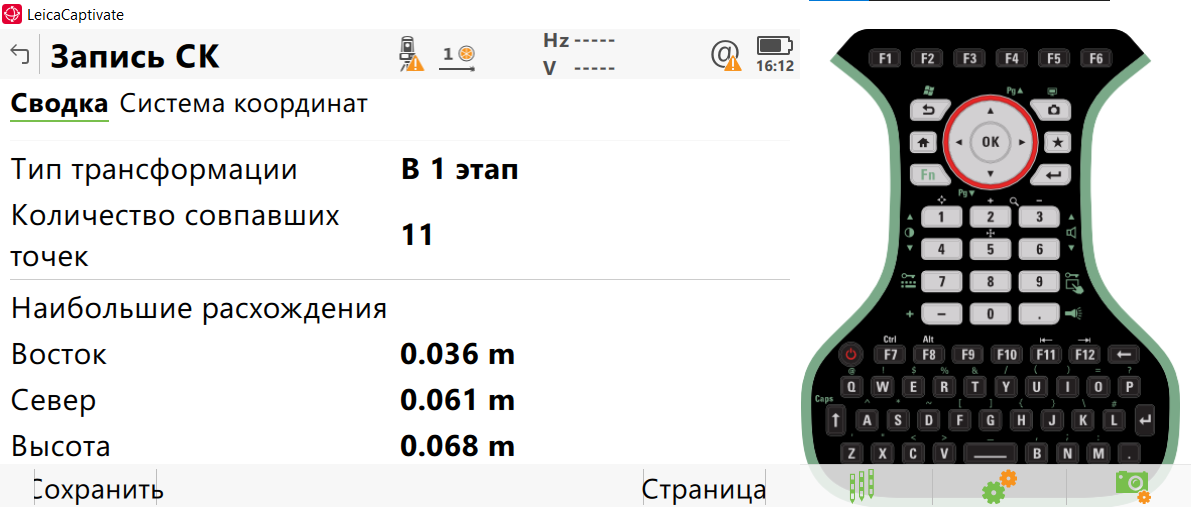
\includegraphics[scale=0.35]{images/25.png}} \\
    Рисунок 25 $-$ Запись СК  
\end{center}
\par Далее представлены «Результаты трансформирования» (рисунок 26), «Результаты СКО (позиционная)» (рисунок 27) и «Результаты СКО (высота)» (рисунок 28).
\begin{center}
    \fbox {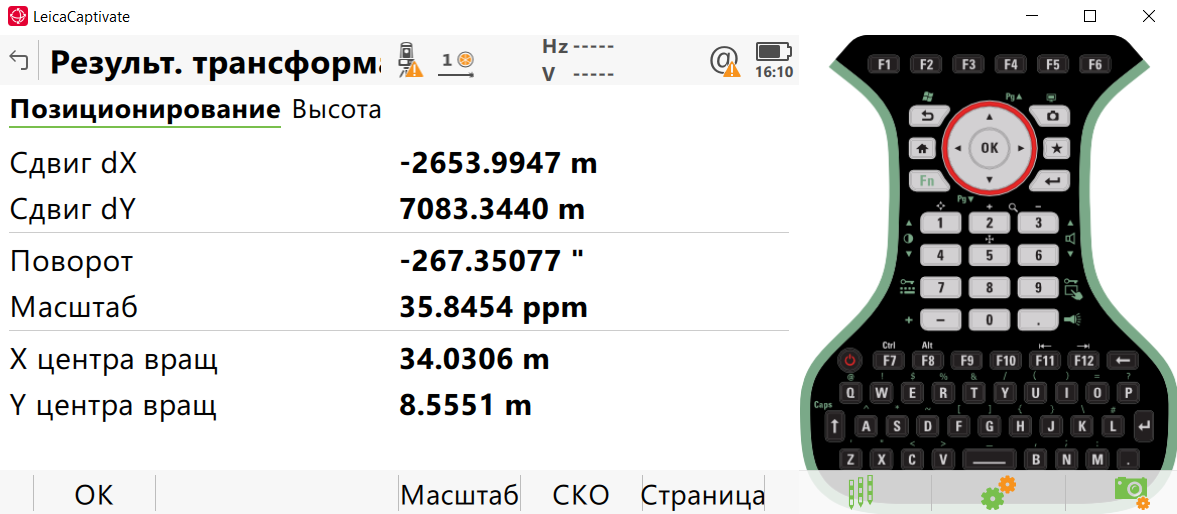
\includegraphics[scale=0.356]{images/26.png}} \\
    Рисунок 26 $-$ Результат трансформирования  
\end{center}
\begin{center}
    \fbox {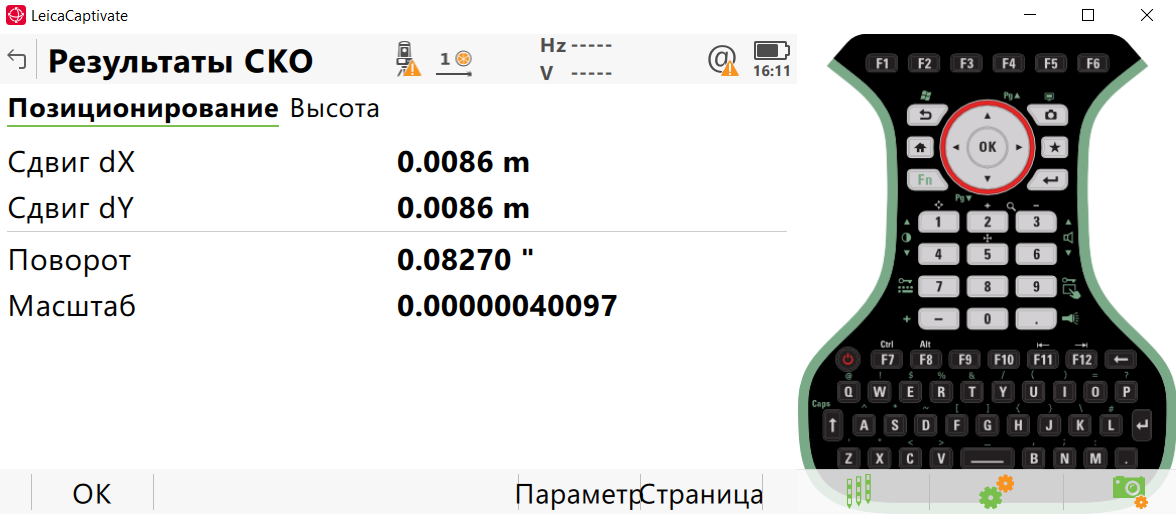
\includegraphics[scale=0.3657]{images/27.png}} \\
    Рисунок 27 $-$ Результаты СКО (позиционная)  
\end{center}
\begin{center}
    \fbox {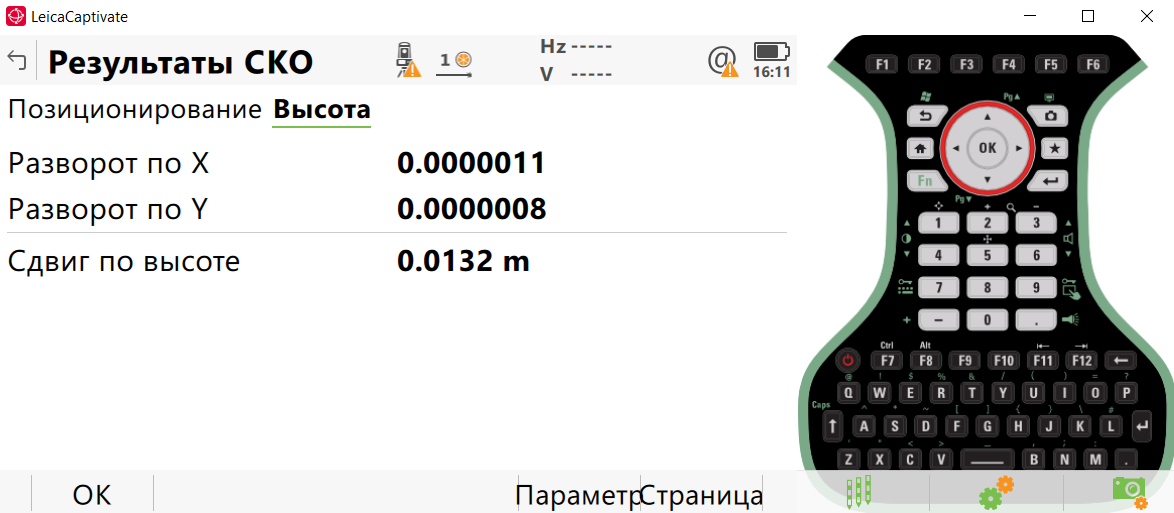
\includegraphics[scale=0.35]{images/28.png}} \\
    Рисунок 28 $-$ Результаты СКО (высота)  
\end{center}
}
\end{document}
